\documentclass[twoside]{book}

% Packages required by doxygen
\usepackage{fixltx2e}
\usepackage{calc}
\usepackage{doxygen}
\usepackage{graphicx}
\usepackage[utf8]{inputenc}
\usepackage{makeidx}
\usepackage{multicol}
\usepackage{multirow}
\PassOptionsToPackage{warn}{textcomp}
\usepackage{textcomp}
\usepackage[nointegrals]{wasysym}
\usepackage[table]{xcolor}

% Font selection
\usepackage[T1]{fontenc}
\usepackage{mathptmx}
\usepackage[scaled=.90]{helvet}
\usepackage{courier}
\usepackage{amssymb}
\usepackage{sectsty}
\renewcommand{\familydefault}{\sfdefault}
\allsectionsfont{%
  \fontseries{bc}\selectfont%
  \color{darkgray}%
}
\renewcommand{\DoxyLabelFont}{%
  \fontseries{bc}\selectfont%
  \color{darkgray}%
}
\newcommand{\+}{\discretionary{\mbox{\scriptsize$\hookleftarrow$}}{}{}}

% Page & text layout
\usepackage{geometry}
\geometry{%
  a4paper,%
  top=2.5cm,%
  bottom=2.5cm,%
  left=2.5cm,%
  right=2.5cm%
}
\tolerance=750
\hfuzz=15pt
\hbadness=750
\setlength{\emergencystretch}{15pt}
\setlength{\parindent}{0cm}
\setlength{\parskip}{0.2cm}
\makeatletter
\renewcommand{\paragraph}{%
  \@startsection{paragraph}{4}{0ex}{-1.0ex}{1.0ex}{%
    \normalfont\normalsize\bfseries\SS@parafont%
  }%
}
\renewcommand{\subparagraph}{%
  \@startsection{subparagraph}{5}{0ex}{-1.0ex}{1.0ex}{%
    \normalfont\normalsize\bfseries\SS@subparafont%
  }%
}
\makeatother

% Headers & footers
\usepackage{fancyhdr}
\pagestyle{fancyplain}
\fancyhead[LE]{\fancyplain{}{\bfseries\thepage}}
\fancyhead[CE]{\fancyplain{}{}}
\fancyhead[RE]{\fancyplain{}{\bfseries\leftmark}}
\fancyhead[LO]{\fancyplain{}{\bfseries\rightmark}}
\fancyhead[CO]{\fancyplain{}{}}
\fancyhead[RO]{\fancyplain{}{\bfseries\thepage}}
\fancyfoot[LE]{\fancyplain{}{}}
\fancyfoot[CE]{\fancyplain{}{}}
\fancyfoot[RE]{\fancyplain{}{\bfseries\scriptsize Generated on Sat Nov 15 2014 17\+:20\+:58 for My Project by Doxygen }}
\fancyfoot[LO]{\fancyplain{}{\bfseries\scriptsize Generated on Sat Nov 15 2014 17\+:20\+:58 for My Project by Doxygen }}
\fancyfoot[CO]{\fancyplain{}{}}
\fancyfoot[RO]{\fancyplain{}{}}
\renewcommand{\footrulewidth}{0.4pt}
\renewcommand{\chaptermark}[1]{%
  \markboth{#1}{}%
}
\renewcommand{\sectionmark}[1]{%
  \markright{\thesection\ #1}%
}

% Indices & bibliography
\usepackage{natbib}
\usepackage[titles]{tocloft}
\setcounter{tocdepth}{3}
\setcounter{secnumdepth}{5}
\makeindex

% Hyperlinks (required, but should be loaded last)
\usepackage{ifpdf}
\ifpdf
  \usepackage[pdftex,pagebackref=true]{hyperref}
\else
  \usepackage[ps2pdf,pagebackref=true]{hyperref}
\fi
\hypersetup{%
  colorlinks=true,%
  linkcolor=blue,%
  citecolor=blue,%
  unicode%
}

% Custom commands
\newcommand{\clearemptydoublepage}{%
  \newpage{\pagestyle{empty}\cleardoublepage}%
}


%===== C O N T E N T S =====

\begin{document}

% Titlepage & ToC
\hypersetup{pageanchor=false,
             bookmarks=true,
             bookmarksnumbered=true,
             pdfencoding=unicode
            }
\pagenumbering{roman}
\begin{titlepage}
\vspace*{7cm}
\begin{center}%
{\Large My Project }\\
\vspace*{1cm}
{\large Generated by Doxygen 1.8.8}\\
\vspace*{0.5cm}
{\small Sat Nov 15 2014 17:20:58}\\
\end{center}
\end{titlepage}
\clearemptydoublepage
\tableofcontents
\clearemptydoublepage
\pagenumbering{arabic}
\hypersetup{pageanchor=true}

%--- Begin generated contents ---
\chapter{Project documentation}
\label{index}\hypertarget{index}{}\hypertarget{index_intro_sec}{}\section{Introduction}\label{index_intro_sec}
This our project documentation. But this project doesn't have any name currently. 
\chapter{Hierarchical Index}
\section{Class Hierarchy}
This inheritance list is sorted roughly, but not completely, alphabetically\+:\begin{DoxyCompactList}
\item Q\+List\+Widget\begin{DoxyCompactList}
\item \contentsline{section}{Detailed\+List}{\pageref{classDetailedList}}{}
\end{DoxyCompactList}
\item Q\+Main\+Window\begin{DoxyCompactList}
\item \contentsline{section}{Main\+Window}{\pageref{classMainWindow}}{}
\end{DoxyCompactList}
\end{DoxyCompactList}

\chapter{Class Index}
\section{Class List}
Here are the classes, structs, unions and interfaces with brief descriptions\+:\begin{DoxyCompactList}
\item\contentsline{section}{\hyperlink{classMainWindow}{Main\+Window} }{\pageref{classMainWindow}}{}
\item\contentsline{section}{\hyperlink{classVariableList}{Variable\+List} \\*A variable list widget }{\pageref{classVariableList}}{}
\end{DoxyCompactList}

\chapter{Class Documentation}
\hypertarget{classDetailedList}{\section{Detailed\+List Class Reference}
\label{classDetailedList}\index{Detailed\+List@{Detailed\+List}}
}


A list widget with details when you click on the title line.  


Inheritance diagram for Detailed\+List\+:\begin{figure}[H]
\begin{center}
\leavevmode
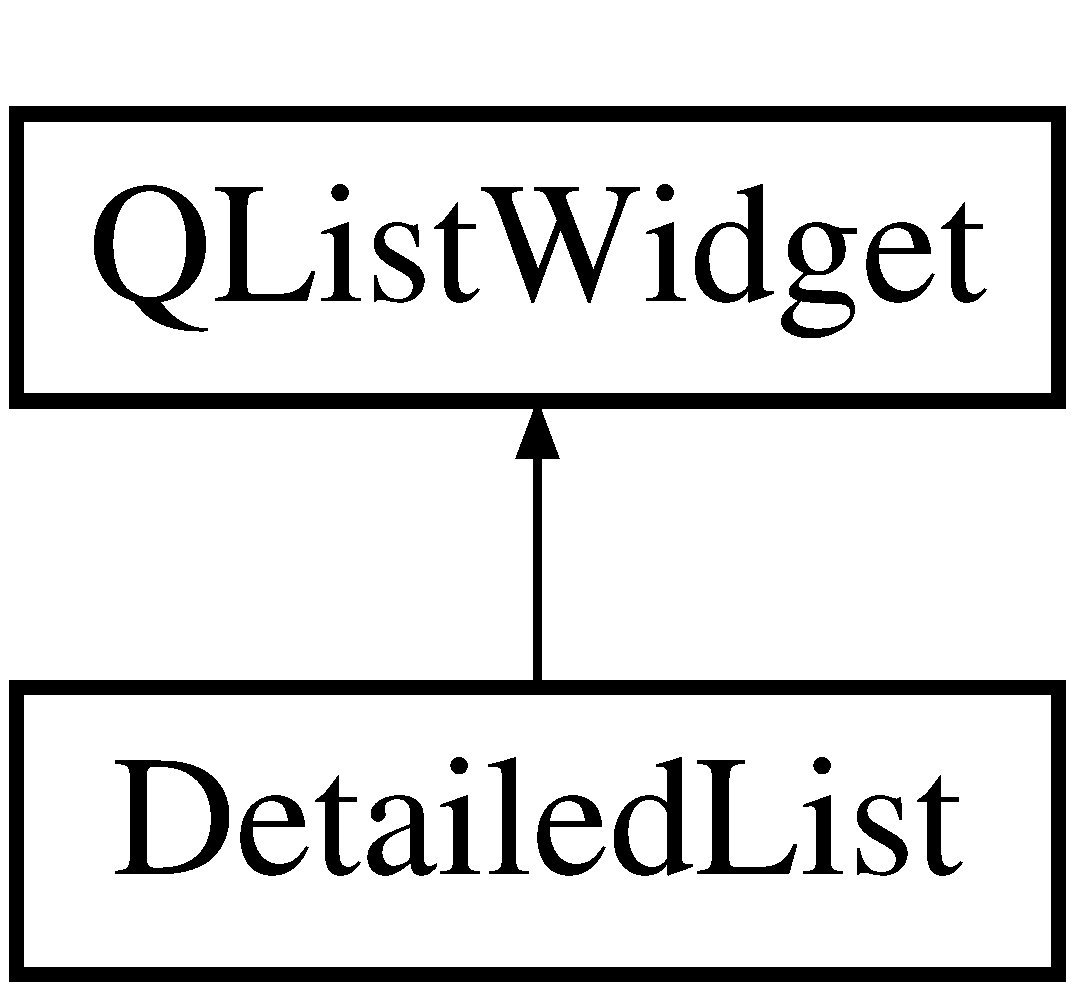
\includegraphics[height=2.000000cm]{classDetailedList}
\end{center}
\end{figure}
\subsection*{Public Slots}
\begin{DoxyCompactItemize}
\item 
\hypertarget{classDetailedList_ad425c5bda6ca07fceee56f1df6ae2cf5}{void {\bfseries D\+E\+B\+U\+Gadd\+New\+Var} ()}\label{classDetailedList_ad425c5bda6ca07fceee56f1df6ae2cf5}

\end{DoxyCompactItemize}
\subsection*{Public Member Functions}
\begin{DoxyCompactItemize}
\item 
\hyperlink{classDetailedList_a82c17dba7dd2bc10317a3b9953cf8943}{Detailed\+List} (Q\+Widget $\ast$parent=0)
\begin{DoxyCompactList}\small\item\em Constructor. \end{DoxyCompactList}\item 
void \hyperlink{classDetailedList_aed40208f4a912b1ecfd3eba7ea2c9233}{add\+Element} (Q\+String title, Q\+String content, bool expanded=true)
\begin{DoxyCompactList}\small\item\em Add a new element to the list. \end{DoxyCompactList}\end{DoxyCompactItemize}
\subsection*{Protected Slots}
\begin{DoxyCompactItemize}
\item 
void \hyperlink{classDetailedList_ad74533c0c6d052007dc282d5b69b83e1}{item\+Clicked} (Q\+List\+Widget\+Item $\ast$clicked)
\begin{DoxyCompactList}\small\item\em Slot triggered when a click is made on an item. \end{DoxyCompactList}\end{DoxyCompactItemize}


\subsection{Detailed Description}
A list widget with details when you click on the title line with a triangle or an arrow that indicate current state. Each element is composed by to Q\+List\+Widget\+Item \+: title and content.

{\bfseries Warning} \+: As each element is indexed by the title name, it has to be unique. 

\subsection{Constructor \& Destructor Documentation}
\hypertarget{classDetailedList_a82c17dba7dd2bc10317a3b9953cf8943}{\index{Detailed\+List@{Detailed\+List}!Detailed\+List@{Detailed\+List}}
\index{Detailed\+List@{Detailed\+List}!Detailed\+List@{Detailed\+List}}
\subsubsection[{Detailed\+List}]{\setlength{\rightskip}{0pt plus 5cm}Detailed\+List\+::\+Detailed\+List (
\begin{DoxyParamCaption}
\item[{Q\+Widget $\ast$}]{parent = {\ttfamily 0}}
\end{DoxyParamCaption}
)\hspace{0.3cm}{\ttfamily [explicit]}}}\label{classDetailedList_a82c17dba7dd2bc10317a3b9953cf8943}
Construct an empty \hyperlink{classDetailedList}{Detailed\+List} with the given {\itshape parent}


\begin{DoxyParams}{Parameters}
{\em parent} & \\
\hline
\end{DoxyParams}


\subsection{Member Function Documentation}
\hypertarget{classDetailedList_aed40208f4a912b1ecfd3eba7ea2c9233}{\index{Detailed\+List@{Detailed\+List}!add\+Element@{add\+Element}}
\index{add\+Element@{add\+Element}!Detailed\+List@{Detailed\+List}}
\subsubsection[{add\+Element}]{\setlength{\rightskip}{0pt plus 5cm}void Detailed\+List\+::add\+Element (
\begin{DoxyParamCaption}
\item[{Q\+String}]{title, }
\item[{Q\+String}]{content, }
\item[{bool}]{expanded = {\ttfamily true}}
\end{DoxyParamCaption}
)}}\label{classDetailedList_aed40208f4a912b1ecfd3eba7ea2c9233}
Add a new element to the list


\begin{DoxyParams}{Parameters}
{\em title} & Plain text title that is allways visible \\
\hline
{\em content} & Rich text content that will be visible when the user click on the line \\
\hline
{\em expanded} & Choose if the new element will be expanded or not \\
\hline
\end{DoxyParams}
\hypertarget{classDetailedList_ad74533c0c6d052007dc282d5b69b83e1}{\index{Detailed\+List@{Detailed\+List}!item\+Clicked@{item\+Clicked}}
\index{item\+Clicked@{item\+Clicked}!Detailed\+List@{Detailed\+List}}
\subsubsection[{item\+Clicked}]{\setlength{\rightskip}{0pt plus 5cm}void Detailed\+List\+::item\+Clicked (
\begin{DoxyParamCaption}
\item[{Q\+List\+Widget\+Item $\ast$}]{clicked}
\end{DoxyParamCaption}
)\hspace{0.3cm}{\ttfamily [protected]}, {\ttfamily [slot]}}}\label{classDetailedList_ad74533c0c6d052007dc282d5b69b83e1}
Slot triggered when a click is made on an item. This is used to expand and reduce elements when you click on a title.


\begin{DoxyParams}{Parameters}
{\em clicked} & A pointer to the clicked item \\
\hline
\end{DoxyParams}


The documentation for this class was generated from the following files\+:\begin{DoxyCompactItemize}
\item 
/home/bob/dev/utt-\/nf05-\/project/sources/detailedlist.\+hpp\item 
/home/bob/dev/utt-\/nf05-\/project/sources/detailedlist.\+cpp\end{DoxyCompactItemize}

\hypertarget{classMainWindow}{\section{Main\+Window Class Reference}
\label{classMainWindow}\index{Main\+Window@{Main\+Window}}
}
Inheritance diagram for Main\+Window\+:\begin{figure}[H]
\begin{center}
\leavevmode
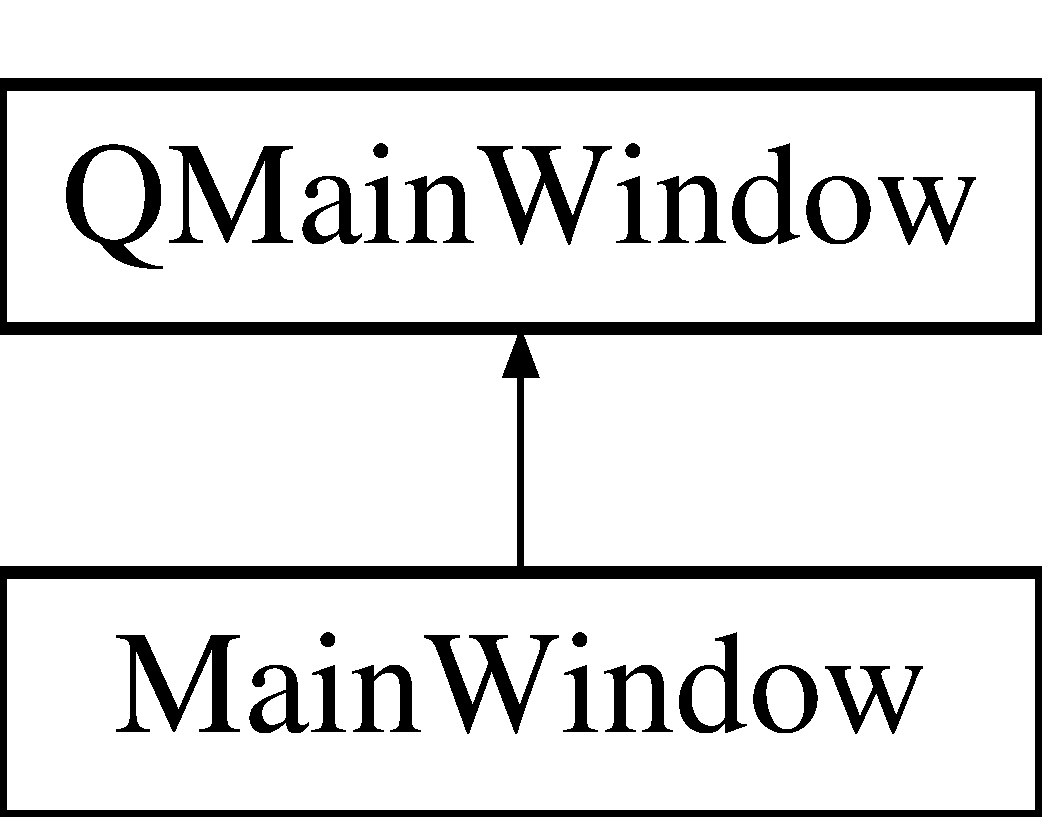
\includegraphics[height=2.000000cm]{classMainWindow}
\end{center}
\end{figure}
\subsection*{Public Member Functions}
\begin{DoxyCompactItemize}
\item 
\hypertarget{classMainWindow_a8b244be8b7b7db1b08de2a2acb9409db}{{\bfseries Main\+Window} (Q\+Widget $\ast$parent=0)}\label{classMainWindow_a8b244be8b7b7db1b08de2a2acb9409db}

\end{DoxyCompactItemize}


The documentation for this class was generated from the following files\+:\begin{DoxyCompactItemize}
\item 
/home/bob/dev/utt-\/nf05-\/project/sources/mainwindow.\+hpp\item 
/home/bob/dev/utt-\/nf05-\/project/sources/mainwindow.\+cpp\end{DoxyCompactItemize}

%--- End generated contents ---

% Index
\newpage
\phantomsection
\addcontentsline{toc}{chapter}{Index}
\printindex

\end{document}
